\documentclass[11pt]{article}
\usepackage{../../latex/stat4ml_style}

\title{Chapter 3: Logistic, Ridge, and Lasso Regression \\ \large Part II --- Introduction to Statistical Learning}
\author{Omid Safarzadeh}
\date{}

\begin{document}
\maketitle

\begin{abstract}
\noindent
This chapter extends linear regression in two directions. \emph{Logistic
regression} swaps the continuous output for a probability, turning the linear
model into a classifier whose loss is cross-entropy. \emph{Ridge} and
\emph{lasso} add a penalty on the coefficients to trade a little bias for a
large cut in variance --- ridge by shrinking every coefficient, lasso by
setting some to exactly zero. We derive each, prove that the logistic loss is
convex (so there is a single optimum), write ridge in closed form, and show
why the lasso's soft-threshold is what produces sparsity.
\end{abstract}

\tableofcontents

% ======================================================================
\section{From a line to a probability, and a penalty on the fit}
% ======================================================================

To classify rather than predict a number, we model the \emph{probability} of
the positive class as a linear function squashed into $(0,1)$ by the
\keyterm{sigmoid} $\sigma(z) = 1/(1+e^{-z})$:
\[
  P(y=1 \mid x) = \sigma(\beta^\top x), \qquad
  \log\frac{P(y=1\mid x)}{P(y=0\mid x)} = \beta^\top x.
\]
The log-odds are linear in $x$, so the decision boundary
$\beta^\top x = 0$ is a hyperplane. Fitting is maximum likelihood, and the
negative log-likelihood is the \keyterm{cross-entropy} loss
\[
  \mathcal{L}(\beta) = -\sum_{i=1}^n \Big[\,y_i \log \sigma(\beta^\top x_i)
     + (1-y_i)\log\big(1 - \sigma(\beta^\top x_i)\big)\Big].
\]

Separately, when predictors are many or collinear, ordinary least squares
overfits. \keyterm{Regularization} adds a penalty on the size of $\beta$:
\[
  \text{ridge: } \min_\beta \|y - X\beta\|^2 + \lambda\|\beta\|_2^2,
  \qquad
  \text{lasso: } \min_\beta \|y - X\beta\|^2 + \lambda\|\beta\|_1.
\]
The squared ($\ell_2$) penalty shrinks coefficients smoothly; the
absolute ($\ell_1$) penalty shrinks them \emph{and} drives small ones to
exactly zero, so the lasso also selects variables. The building blocks are
short:

\begin{lstlisting}[language=Python]
import math

def sigmoid(z):
    return 1.0 / (1.0 + math.exp(-z))

def cross_entropy(y, p):                       # one observation
    return -(y * math.log(p) + (1 - y) * math.log(1 - p))

def soft_threshold(z, lam):                    # the lasso's shrinkage
    if z >  lam: return z - lam
    if z < -lam: return z + lam
    return 0.0

print(round(sigmoid(0.0), 3))                  # 0.5
print(round(cross_entropy(1, 0.9), 4))         # 0.1054
print(soft_threshold(0.7, 1.0), soft_threshold(2.0, 1.0))  # 0.0 1.0
\end{lstlisting}

\noindent The figure shows both ideas: a logistic decision boundary
separating two classes, and the three shrinkage rules side by side --- OLS
leaves a coefficient alone, ridge scales it down, and the lasso's
soft-threshold flattens a whole band around zero flat to zero.

\begin{figure}[h]
  \centering
  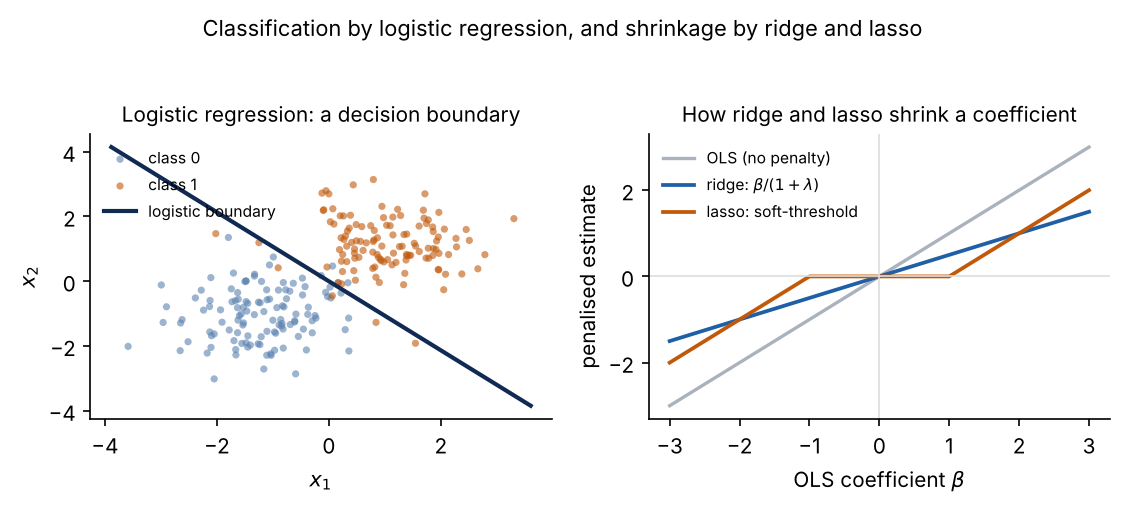
\includegraphics[width=\linewidth]{figures/logreg_panel.png}
\end{figure}

% ======================================================================
\section{Why these fits are well-behaved}
% ======================================================================

\begin{theorem}[The logistic loss is convex]
The cross-entropy $\mathcal{L}(\beta)$ is convex in $\beta$; its Hessian is
positive semidefinite.
\end{theorem}
\begin{proof}
Let $p_i = \sigma(\beta^\top x_i)$. The gradient is
$\nabla\mathcal{L} = \sum_i (p_i - y_i)\,x_i = X^\top(p - y)$, and since
$\sigma'(z) = \sigma(z)(1-\sigma(z))$, the Hessian is
\[
  \nabla^2 \mathcal{L} = \sum_{i} p_i(1-p_i)\, x_i x_i^\top = X^\top S X,
  \qquad S = \operatorname{diag}\big(p_i(1-p_i)\big).
\]
Each $p_i(1-p_i) \ge 0$, so $S \succeq 0$ and $X^\top S X \succeq 0$. A
twice-differentiable function with a positive-semidefinite Hessian is convex,
so the loss has no local minima to get stuck in --- gradient descent finds
the global optimum.
\end{proof}

Ridge, unlike the lasso, has a closed form, and it fixes a failure of OLS.

\begin{theorem}[Ridge solution]
$\hat\beta_{\text{ridge}} = (X^\top X + \lambda I)^{-1} X^\top y$, and the
matrix $X^\top X + \lambda I$ is invertible for every $\lambda > 0$ even when
$X^\top X$ is singular.
\end{theorem}
\begin{proof}
Differentiate $\|y-X\beta\|^2 + \lambda\|\beta\|^2$ and set to zero:
$-2X^\top(y - X\beta) + 2\lambda\beta = 0$, giving
$(X^\top X + \lambda I)\beta = X^\top y$. For any $\lambda>0$ the matrix
$X^\top X + \lambda I$ has all eigenvalues $\ge \lambda > 0$ (those of
$X^\top X$ are $\ge 0$), so it is invertible --- ridge is defined even with
more predictors than observations.
\end{proof}

The lasso has no such formula in general, but for one coordinate at a time it
does, and that formula is exactly the soft-threshold.

\begin{theorem}[Lasso's soft-threshold]
Minimising $\tfrac12(z - \beta)^2 + \lambda|\beta|$ over $\beta$ gives
$\hat\beta = S_\lambda(z) = \operatorname{sign}(z)\,\max(|z|-\lambda,\,0)$.
\end{theorem}
\begin{proof}
For $\beta>0$ the objective is smooth with derivative $\beta - z + \lambda$,
zero at $\beta = z-\lambda$ (valid when $z>\lambda$); for $\beta<0$ similarly
$\beta = z+\lambda$ (valid when $z<-\lambda$). When $|z|\le\lambda$ the
subgradient of $|\beta|$ at $0$ is the interval $[-1,1]$ and $0 \in
[z-\lambda,\,z+\lambda]$, so $\hat\beta=0$. Collecting the cases gives
$S_\lambda(z)$ --- which is zero on a whole band $|z|\le\lambda$, and that
flat band is where sparsity comes from.
\end{proof}

% ======================================================================
\section{The geometry of sparsity, and beyond}
% ======================================================================

Why does $\ell_1$ zero coefficients out while $\ell_2$ does not? The penalty
$\|\beta\|_1 \le t$ is a diamond with corners on the axes, while
$\|\beta\|_2 \le t$ is a round ball. The least-squares contours first touch
the diamond at a corner --- where some coordinates are exactly zero ---
whereas they touch the ball on a smooth face, where no coordinate is exactly
zero. Sparsity is a consequence of the corners.

The absolute value is not differentiable at zero, so there is no neat normal
equation; the optimum is characterised by \keyterm{subgradients} (the
$[-1,1]$ interval used above) and computed by \keyterm{coordinate descent},
which applies the soft-threshold to one coefficient at a time until nothing
moves. The \keyterm{elastic net} combines both penalties,
$\lambda\big(\alpha\|\beta\|_1 + (1-\alpha)\|\beta\|_2^2\big)$, keeping the
lasso's selection while handling groups of correlated predictors more
gracefully. All of this buys variance reduction at the price of a little
bias --- the same trade-off of Chapter 2, now controlled by $\lambda$.

\begin{summarybox}
Logistic regression models $P(y=1\mid x) = \sigma(\beta^\top x)$ and is fit by
minimising the convex cross-entropy loss (Hessian $X^\top S X \succeq 0$).
Ridge adds $\lambda\|\beta\|_2^2$, with closed form
$(X^\top X + \lambda I)^{-1}X^\top y$ that is always invertible; the lasso adds
$\lambda\|\beta\|_1$, whose per-coordinate solution is the soft-threshold
$S_\lambda(z)=\operatorname{sign}(z)\max(|z|-\lambda,0)$, zeroing small
coefficients and so selecting variables. The $\ell_1$ corners are the
geometric reason for sparsity.
\end{summarybox}

\end{document}
